\documentclass[slidestop,compress,mathserif]{beamer}
\usepackage{xeCJK}
\usepackage{amsmath}
\usepackage{changepage}
\usepackage{indentfirst} 
\setlength{\parindent}{2em}
\setCJKmainfont{SimSun}
\usetheme{default}

\renewcommand{\today}{\number\year 年\number\month 月\number\day 日}

\title{MaxClique}
\author{曾奥涵 \texttt{2018013383}\\刘润达 \texttt{2018013412}}
%\institute{计 86}

\begin{document}
	\setlength{\baselineskip}{20pt}
	\begin{frame}
		\titlepage
	\end{frame}
	
	\begin{frame}
		\frametitle {介绍}
		给定图 $G$,图中的一个团是 $G$ 的一个完全子图,其中任意两个节点之间都有边连接。求给定图中最大团的问题被称为最大团问题。最大团问题是经典的 NP-hard 问题,现如今解决最大团问题的算法主要分为两类:
		
		\begin{itemize}
			\item 确定性算法
			\item 启发式算法
		\end{itemize}		
		
		我们组同时实现了两种确定性算法 MaxCLQ 和 BBMCX,一种启发式算法 DLS。其中我们实现的经过优化后的 BBMCX 算法效率在一定程度上优于论文中的 BBMCX 算法(BBMCX 算法已是目前最快的确定性算法) 。
	
	\end{frame}
	
	\begin{frame}
		\frametitle {确定性算法}
			我们实现了两种确定性算法	
			\begin{itemize}
				\item MaxCLQ
				\item BBMCX
			\end{itemize}
			
			在 BBMCX 的基础之上,我们加入了两个优化:
			
			\begin{itemize}
				\item 用 \texttt{std::bitset} 高效维护节点集合
				\item 在染色过程中启发式地对节点重排序
			\end{itemize}
			
			最终实现的算法名为 BBMCX\_BITSET。

	\end{frame}
		
	\begin{frame}
		\frametitle {BBMCX - 用 \texttt{std::bitset} 维护节点集合}
	 	在 BBMCX 的算法执行过程中,需要寻找包含三个颜色的集合。对于点 $v$,第一个颜色的成立条件是存在颜色 $k_1$,使得 $|C_{k_1} \cap N(v)| = 1$,记重合的元素为 $w$。第二个颜色的成立条件是存在颜色 $k_2$,$|C_{k_2} \cap N(v) \cap N(w)| = 0$。
	
	条件中涉及大量的集合运算,如果单纯采用 \texttt{vector} 维护节点集合,只能遍历的形式来判断,单次复杂度为 $O(|V|)$。我们在染色的过程中,用 \texttt{std::bitset} 动态维护每个颜色对应的节点集合,同时预处理出每个节点相邻节点的 \texttt{bitset},这样就能够高效的利用 \texttt{bitset} 按位并行计算的优势判断成立条件,复杂度降为 $O(\frac {|V|} {64})$。加入该优化,算法能有接近 $50\%$ 的性能提升。
	\end{frame}
	
	\begin{frame}
		\frametitle{BBMCX - 启发式节点排序}
	
		在染色的过程中,如果能够按照节点度数从大到小的顺序依次染色,那么会得到更好的染色结果。论文中提出的排序方式是:找到一个度数最小的点,将点从图中删掉,再找图中最小的点。然而,这种方案对于节点集合 $V$ 的导出子图而言,重新排序的代价是 $O(|G_V|^2)$,复杂度较高。Janez Konc 等人分析得出,只有在搜索树的最浅几层重新计算节点才是划算的\footnote{Konc, J., Janečič, D.; An improved branch and bound algorithm for the maximum clique problem. MATCH Commun. Math. Comput. Chem. 58: 569-590, 2007}。
		
		于是我们提出这样一种策略,根据输入数据的规模,动态计算重排序的阈值 $k$,在搜素树中 $< k$ 的所有层重新计算节点顺序,$\ge k$ 的所有层按照原先的顺序排序。该优化加入后,搜索树的大小有了一定的减小,总的计算效率得到了一定的提升。
	
	\end{frame}
	
	\begin{frame}
	\frametitle{启发式节点排序}
		我们分析发现,上述策略的瓶颈就在于重排导出子图的代价较高。我们考虑退而求其次,直接以节点在导出子图中的度数大小排序,这样的策略在单层效果上会劣于依次删点排序,然而,利用 \texttt{bitset},导出子图的节点度数可以在 $O(\frac {|G_v|^2} {64})$ 的复杂度内计算完成,这样重排的复杂度就不再成为瓶颈。
		
		我们采用新的排序策略:根据图大小设定阈值 $k$,在搜素树中 $< k$ 的所有层采用删点策略计算顺序,$\ge k$ 的所有层直接按照导出子图中的点度排序。
		
		该优化加入后,搜索树的大小大大减小,算法的性能约有 $100\%$ 的提升(详见实验部分)。
	\end{frame}
	
	\begin{frame}
		\frametitle {启发式算法}
			我们实现了一种启发式算法 DLS(Dynamic Local Search)。
			
			DLS 算法采用扩展(expand)和平移(plateauSearch)两种方式对当前团进行扩展。通过引入 Penalty 机制来减少算法困在局部最优解的情况,同时维护一个 DLS 数据结构,保证集合增删过程中的高效性。
			
			最终结果在较小的测试点上表现不佳,但在非常大的测试点上,DLS 算法能够在相对较短的时间内计算出一个较优解。
		
	\end{frame}

	\begin{frame}
\frametitle {实验结果}
\vspace{1em}
	\begin{adjustwidth}{-2em}{-2em}
		\begin{table}[H]
	\begin{center}
		\begin{tabular}{c|c|c|c|c|c}
			\textbf{Name} & $\omega$ & \textbf{MaxCLQ} & \textbf{BBMCX} & \textbf{BBMCX\_B} & \textbf{DLS}\\
			\hline
brock200\_1 & 21 & 5.848s & 1.377s & \textbf{0.284s} & 3.95s(21) \\
brock200\_2 & 12 & 0.131s & 0.027s & \textbf{0.005s} & 3.27s(10)  \\
brock200\_3 & 15 & 0.365s & 0.092s & \textbf{0.015s} & 3.77s(14)   \\
brock200\_4 & 17 & 1.18s & 0.336s & \textbf{0.059s} & 5.12s(17)   \\
brock400\_1 & 27 & 5614.92s & 586.18s & \textbf{171.73s} & 15.82s(23) \\
brock400\_2 & 29 & 2118.35s & 242.39s & \textbf{68.01s} & 24.95s(24) \\
brock400\_3 & 31 & 3623.74s & 386.20s & \textbf{110.60s} & 30.37s(23)\\
brock400\_4 & 33 & 2082.06s & 207.90s & \textbf{61.54s} & 14.99s(24)\\
brock800\_1 & 23 & $>12h$ & 7342.49s & \textbf{2475.67s} & 31.22s(20)\\
brock800\_2 & 24 & $>12h$ & 9229.95s & \textbf{2153.64s} & 29.19s(20)\\
brock800\_3 & 25 & $>12h$ & 7183.32s & \textbf{1526.52s} & 25.73s(19)\\
brock800\_4 & 26 & $>12h$ & 8257.82s & \textbf{1030.65s} & 24.88s(18)\\
frp100-40 & 100 & $12h(80)$ & $12h(82)$ & $12h(83)$ & \textbf{1h(84)}
		\end{tabular}
		\caption{在不同的数据集上,各算法的用时对比}
	\end{center}
		\end{table}
	\end{adjustwidth}
	\end{frame}
	
	\begin{frame}
\frametitle {实验结果}
\vspace{1em}
	\begin{adjustwidth}{-2em}{-2em}
		\begin{table}[H]
	\begin{center}
		\begin{tabular}{c|c|c|c|c|c}
			\textbf{Name} & $\omega$ & \textbf{BBMCX\_1} & \textbf{BBMCX\_2}\\
			\hline
brock200\_1 & 21 & 0.409s & \textbf{0.284s} \\
brock200\_2 & 12 & 0.008s & \textbf{0.005s} \\
brock200\_3 & 15 & 0.023s & \textbf{0.015s} \\
brock200\_4 & 17 & 0.076s & \textbf{0.059s} \\
brock400\_1 & 27 & 345.48s & \textbf{171.73s} \\
brock400\_2 & 29 & 128.36s & \textbf{68.01s} \\
brock400\_3 & 31 & 218.69s & \textbf{110.60s} \\
brock400\_4 & 33 & 153.17s & \textbf{61.54s} \\
brock800\_1 & 23 & 6821.66s & \textbf{2475.67s} \\
brock800\_2 & 24 & 7210.39s & \textbf{2153.64s} \\
brock800\_3 & 25 & 5525.27s & \textbf{1526.52s} \\
brock800\_4 & 26 & 6219.36s & \textbf{1030.65s}
		\end{tabular}
		\caption{启发式重排序策略用时对比}
	\end{center}
		\end{table}
	\end{adjustwidth}
	\end{frame}

	
	\begin{frame}
%	\vspace{-2em}
\frametitle {实验结果}
\vspace{1em}
	\begin{adjustwidth}{-2em}{-2em}
		\begin{table}[H]
	\begin{center}
		\begin{tabular}{c|c|c|c|c|c}
			\textbf{Name} & $\omega$ & \textbf{BBMCX} & \textbf{Ours}\\
			\hline
brock200\_1 & 21 & \textbf{0.240s} & 0.284s \\
brock200\_2 & 12 & 0.008s & \textbf{0.005s} \\
brock200\_3 & 15 & 0.018s & \textbf{0.015s} \\
brock200\_4 & 17 & \textbf{0.044s} & 0.059s \\
brock400\_1 & 27 & 194.7s & \textbf{171.73s} \\
brock400\_2 & 29 & 87.94s & \textbf{68.01s} \\
brock400\_3 & 31 & 155.5s & \textbf{110.60s} \\
brock400\_4 & 33 & 88.87s & \textbf{61.54s} \\
brock800\_1 & 23 & 3496.9s  & \textbf{2475.67s} \\
brock800\_2 & 24 & 3140.1s & \textbf{2153.64s} \\
brock800\_3 & 25 & 2063.7s & \textbf{1526.52s} \\
brock800\_4 & 26 & 1429.8s & \textbf{1030.65s}
		\end{tabular}
		\caption{与论文中的实现对比}
	\end{center}
		\end{table}
	\end{adjustwidth}
	\end{frame}
	
	\begin{frame}
		\frametitle {Github 协作}
		\begin{figure}[H]
		\centering
		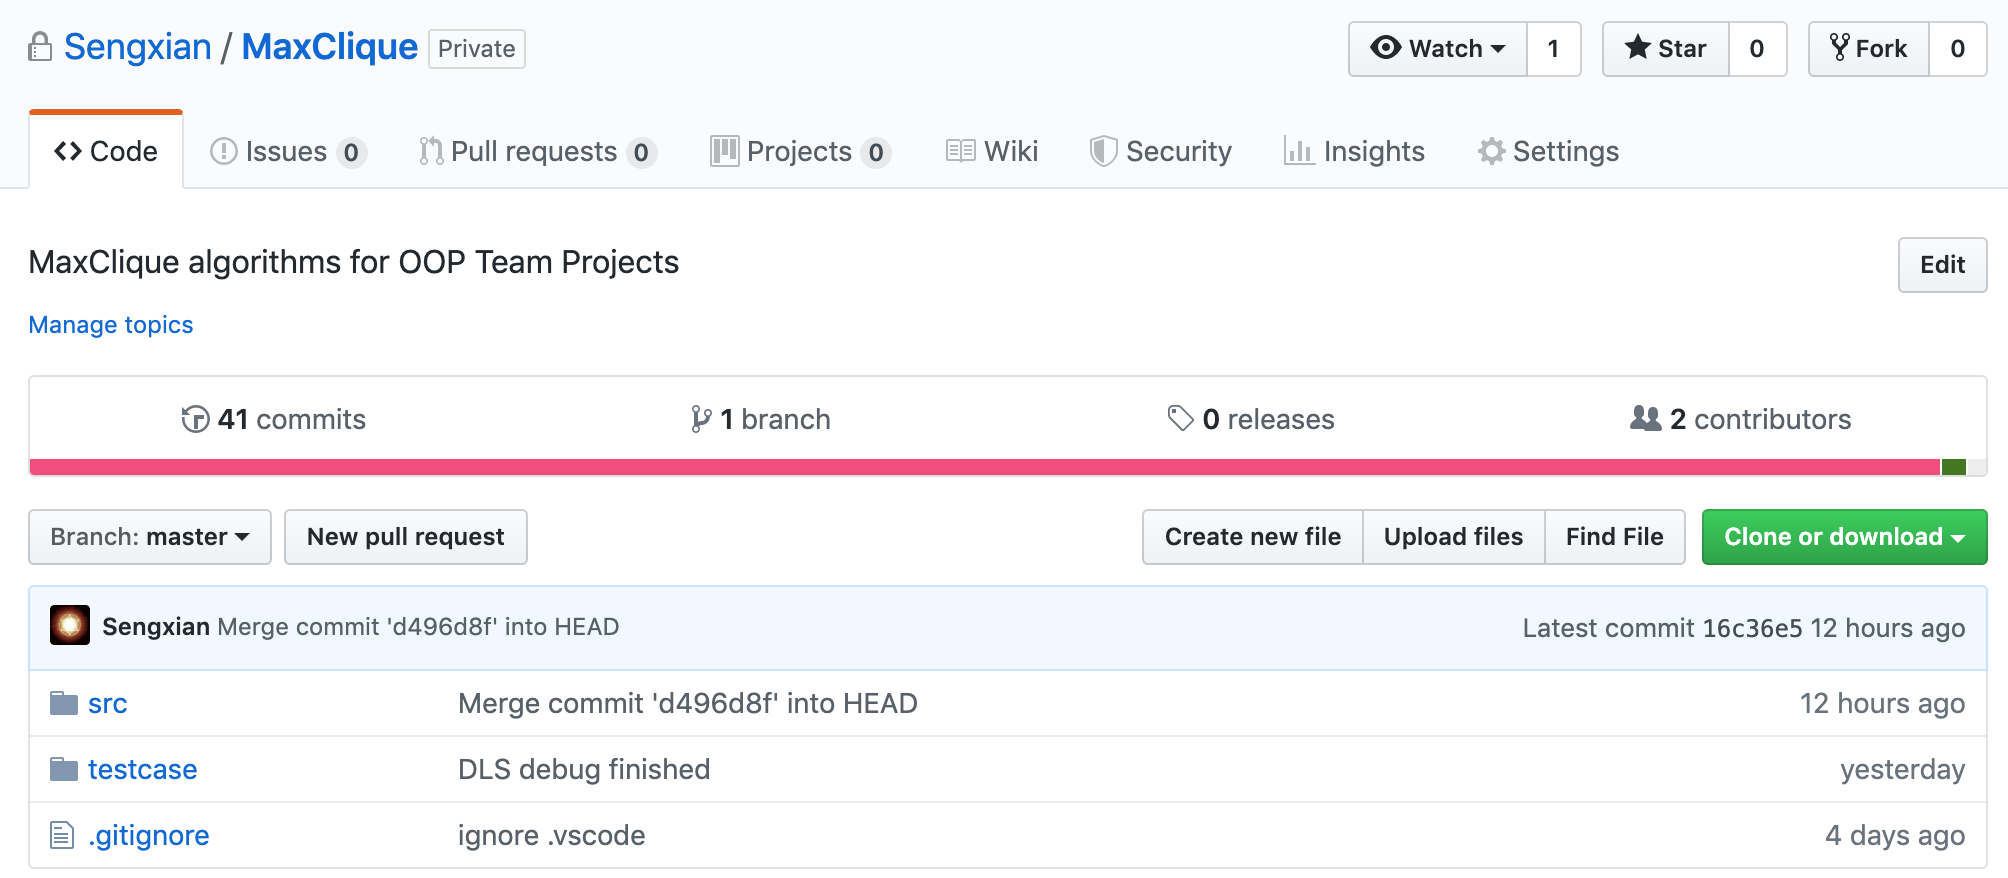
\includegraphics[width=0.9\textwidth]{./github.png}
		\end{figure}
		小组采用 Github 协作,开发效率较高。
	\end{frame}
\end{document}
